\subsection{Sensor}

%\subsection{Design Requirements:}

\textbf{Background}\\
Blah Blah Blah some background

\textbf{Design Specification}\\

% Table generated by Excel2LaTeX from sheet 'Sheet1'
\begin{table}[htbp]
  \centering
  \caption{Add caption}
\resizebox{\textwidth}{!}{\begin{tabular}{lccll}
\hline
    \multicolumn{1}{c}{Requirement} & Wish/Deman & \multicolumn{1}{p{10.785em}}{Importance} & \multicolumn{1}{c}{Engineering Specification} & \multicolumn{1}{c}{Target Value} \\
          &       & \multicolumn{1}{p{8.785em}}{ (1 low, 5 high)} &       &  \\
\hline
    Sensors open to atmosphere & D     &       &       &  \\
    Water Proof & D     &       & IP67  &  \\
    Long battery life & W     & 4     & Self powered + battery capacity. & 1 week battery life \\
    Easy to set up & W     & 5     &       &  \\
    Durable & W     & 4     & Sustain accidental drops from height & 0.5m \\
    Low cost & W     & 3     & Component and raw material cost & £200 \\
    Recylable & W     & 2     &       &  \\
    Transparent & W     & 4     &       &  \\
    Easy to charge & W     & 2     & Clear acess to charging port &  \\
    Cheap to manufacture & W     & 3     & Manufacture and assembly cost & £30 \\
    Small form factor & W     & 3     & Overall dimmensions & 30x30x30cm \\
\hline
    \end{tabular}}%
  \label{tab:addlabel}%
\end{table}%

Long Battery Life (4):\\
To ensure regular air quality measurements minimum intervention with the device is required. The most involved element is the charging of the device, therefore this should be kept to a minimum by having a long battery life.
\vskip 0.1in
Easy to set up (5):\\
Crucial to ensuring a citizen science approach to monitoring air quality is maintaining a very simple set up of the sensor. As stipulated in the background the device must be portable and thus require 'packing up' and 'setting up'. Therefor both of these processes must be intuitive (completable without any training or instruction).
\vskip 0.1in
Durable (4):\\
Due to the protable nature of the sensor, and to ensure longevity, the device must be durable to general wear and tear. This has the added benefit of reducing the cost of the airmonitoring system by extending the useable life of each sensor.
\vskip 0.1in
Low Cost (3:)\\
\vskip 0.1in
Recylable (2):\\
\vskip 0.1in
Transparent (4):\\
\vskip 0.1in
Easy to charge (2):\\
\vskip 0.1in
Cheap to manufacture (3):\\
\vskip 0.1in
Small form factor (3):\\
\vskip 0.1in

\textbf{Concepts}\\

\begin{figure}[H]
\centering
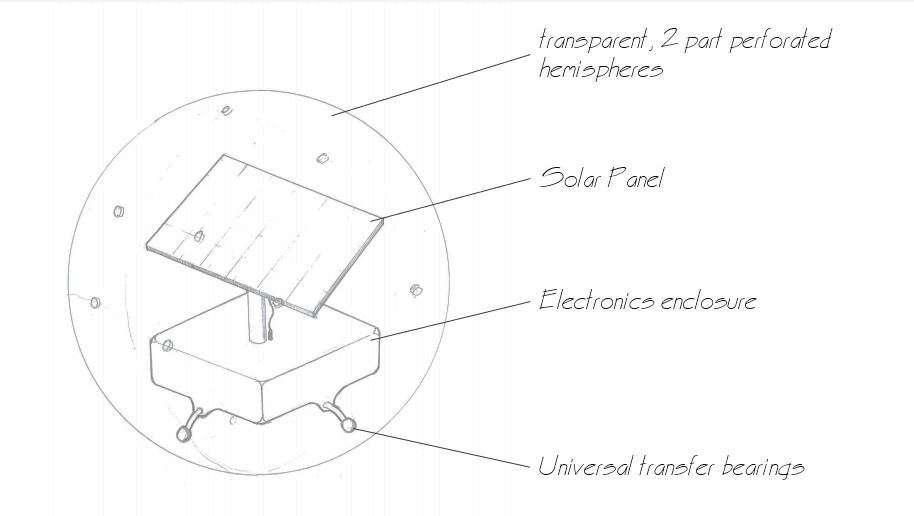
\includegraphics[width=0.9\linewidth]{Engineering_hardware/Engineering_hardware_Figures/Concept_ball.JPG}
\caption{Inspection of Wagons during Operation "Davey Jones Locker" Showing 150mm Poison gas shell. From Arison III H. L. (2013) with permission \cite{arison2014european}.  }
\label{fig:15cm_shell_loading}
\end{figure}



\begin{figure}[H]
\centering
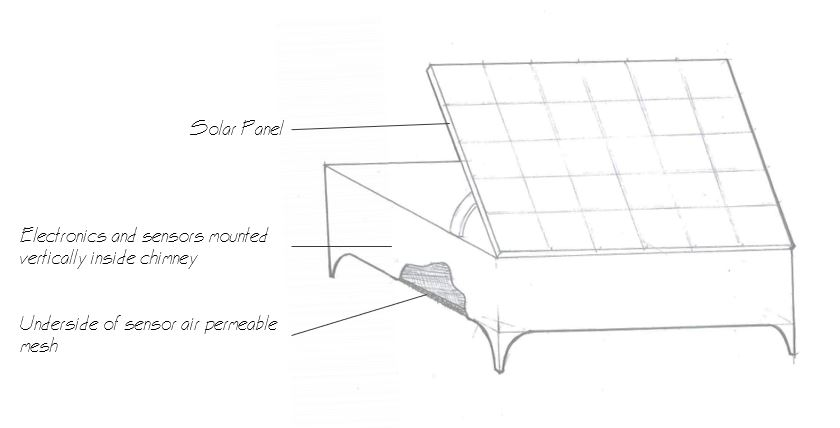
\includegraphics[width=0.8\linewidth]{Engineering_hardware/Engineering_hardware_Figures/Concept_box.JPG}
\caption{Inspection of Wagons during Operation "Davey Jones Locker" Showing 150mm Poison gas shell. From Arison III H. L. (2013) with permission \cite{arison2014european}.  }
\label{fig:15cm_shell_loading}
\end{figure}


\begin{figure}[H]
\centering
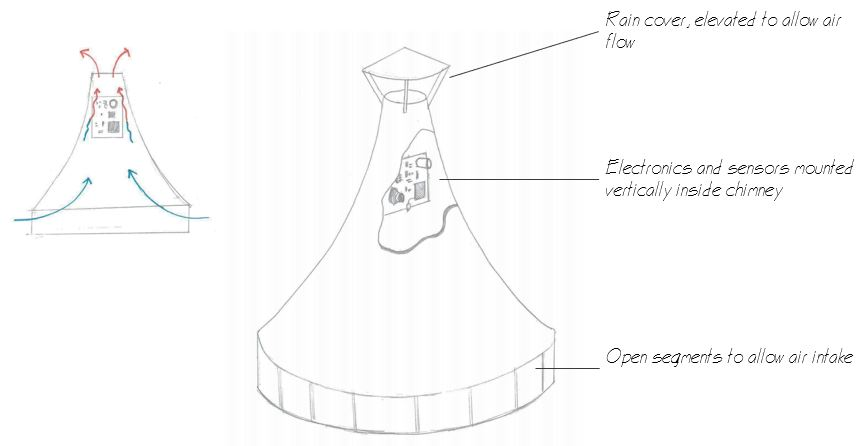
\includegraphics[width=0.8\linewidth]{Engineering_hardware/Engineering_hardware_Figures/Concept_chimney.JPG}
\caption{Inspection of Wagons during Operation "Davey Jones Locker" Showing 150mm Poison gas shell. From Arison III H. L. (2013) with permission \cite{arison2014european}.  }
\label{fig:15cm_shell_loading}
\end{figure}


\begin{figure}[H]
\centering
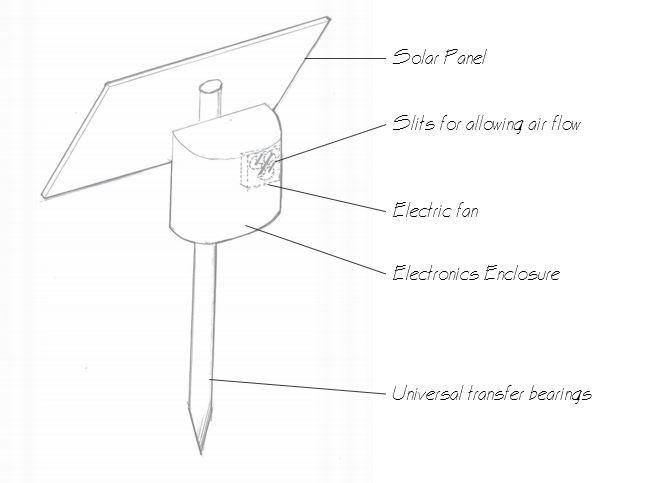
\includegraphics[width=0.6\linewidth]{Engineering_hardware/Engineering_hardware_Figures/Concept_stake.JPG}
\caption{Inspection of Wagons during Operation "Davey Jones Locker" Showing 150mm Poison gas shell. From Arison III H. L. (2013) with permission \cite{arison2014european}.  }
\label{fig:15cm_shell_loading}
\end{figure}

Pair wise comparison: or just weighted scoring

% Table generated by Excel2LaTeX from sheet 'Sheet1'
\begin{table}[htbp]
  \centering
  \caption{Add caption}
    \begin{tabular}{lrrrr}
          & \multicolumn{4}{c}{Concepts} \\
\hline
    Spec No. & \multicolumn{1}{l}{A} & \multicolumn{1}{l}{B} & \multicolumn{1}{l}{C} & \multicolumn{1}{l}{D} \\
\hline
    \multicolumn{1}{r}{1} & 1     & 1     & 1     & 1 \\
    \multicolumn{1}{r}{2} & 1     & 1     & 1     & 1 \\
    \multicolumn{1}{r}{3} & 3     & 5     & 2     & 4 \\
    \multicolumn{1}{r}{4} & 5     & 4     & 3     & 1 \\
    \multicolumn{1}{r}{5} & 5     & 3     & 4     & 3 \\
    \multicolumn{1}{r}{6} & 4     & 5     & 2     & 3 \\
    \multicolumn{1}{r}{7} & 3     & 3     & 3     & 3 \\
    \multicolumn{1}{r}{8} & 5     & 4     & 5     & 3 \\
    \multicolumn{1}{r}{9} & 3     & 5     & 3     & 4 \\
    \multicolumn{1}{r}{10} & 3     & 4     & 2     & 3 \\
    \multicolumn{1}{r}{11} & 4     & 4     & 3     & 2 \\
    weighted sum & \cellcolor[rgb]{ .388,  .745,  .482}127 & \cellcolor[rgb]{ .427,  .757,  .486}126 & \cellcolor[rgb]{ .98,  .616,  .459}96 & \cellcolor[rgb]{ .973,  .412,  .42}86 \\
\hline
    \end{tabular}%
  \label{tab:addlabel}%
\end{table}%



%prototypes for each mechanism:
%locking two parts together


\textbf{Prototype}\\

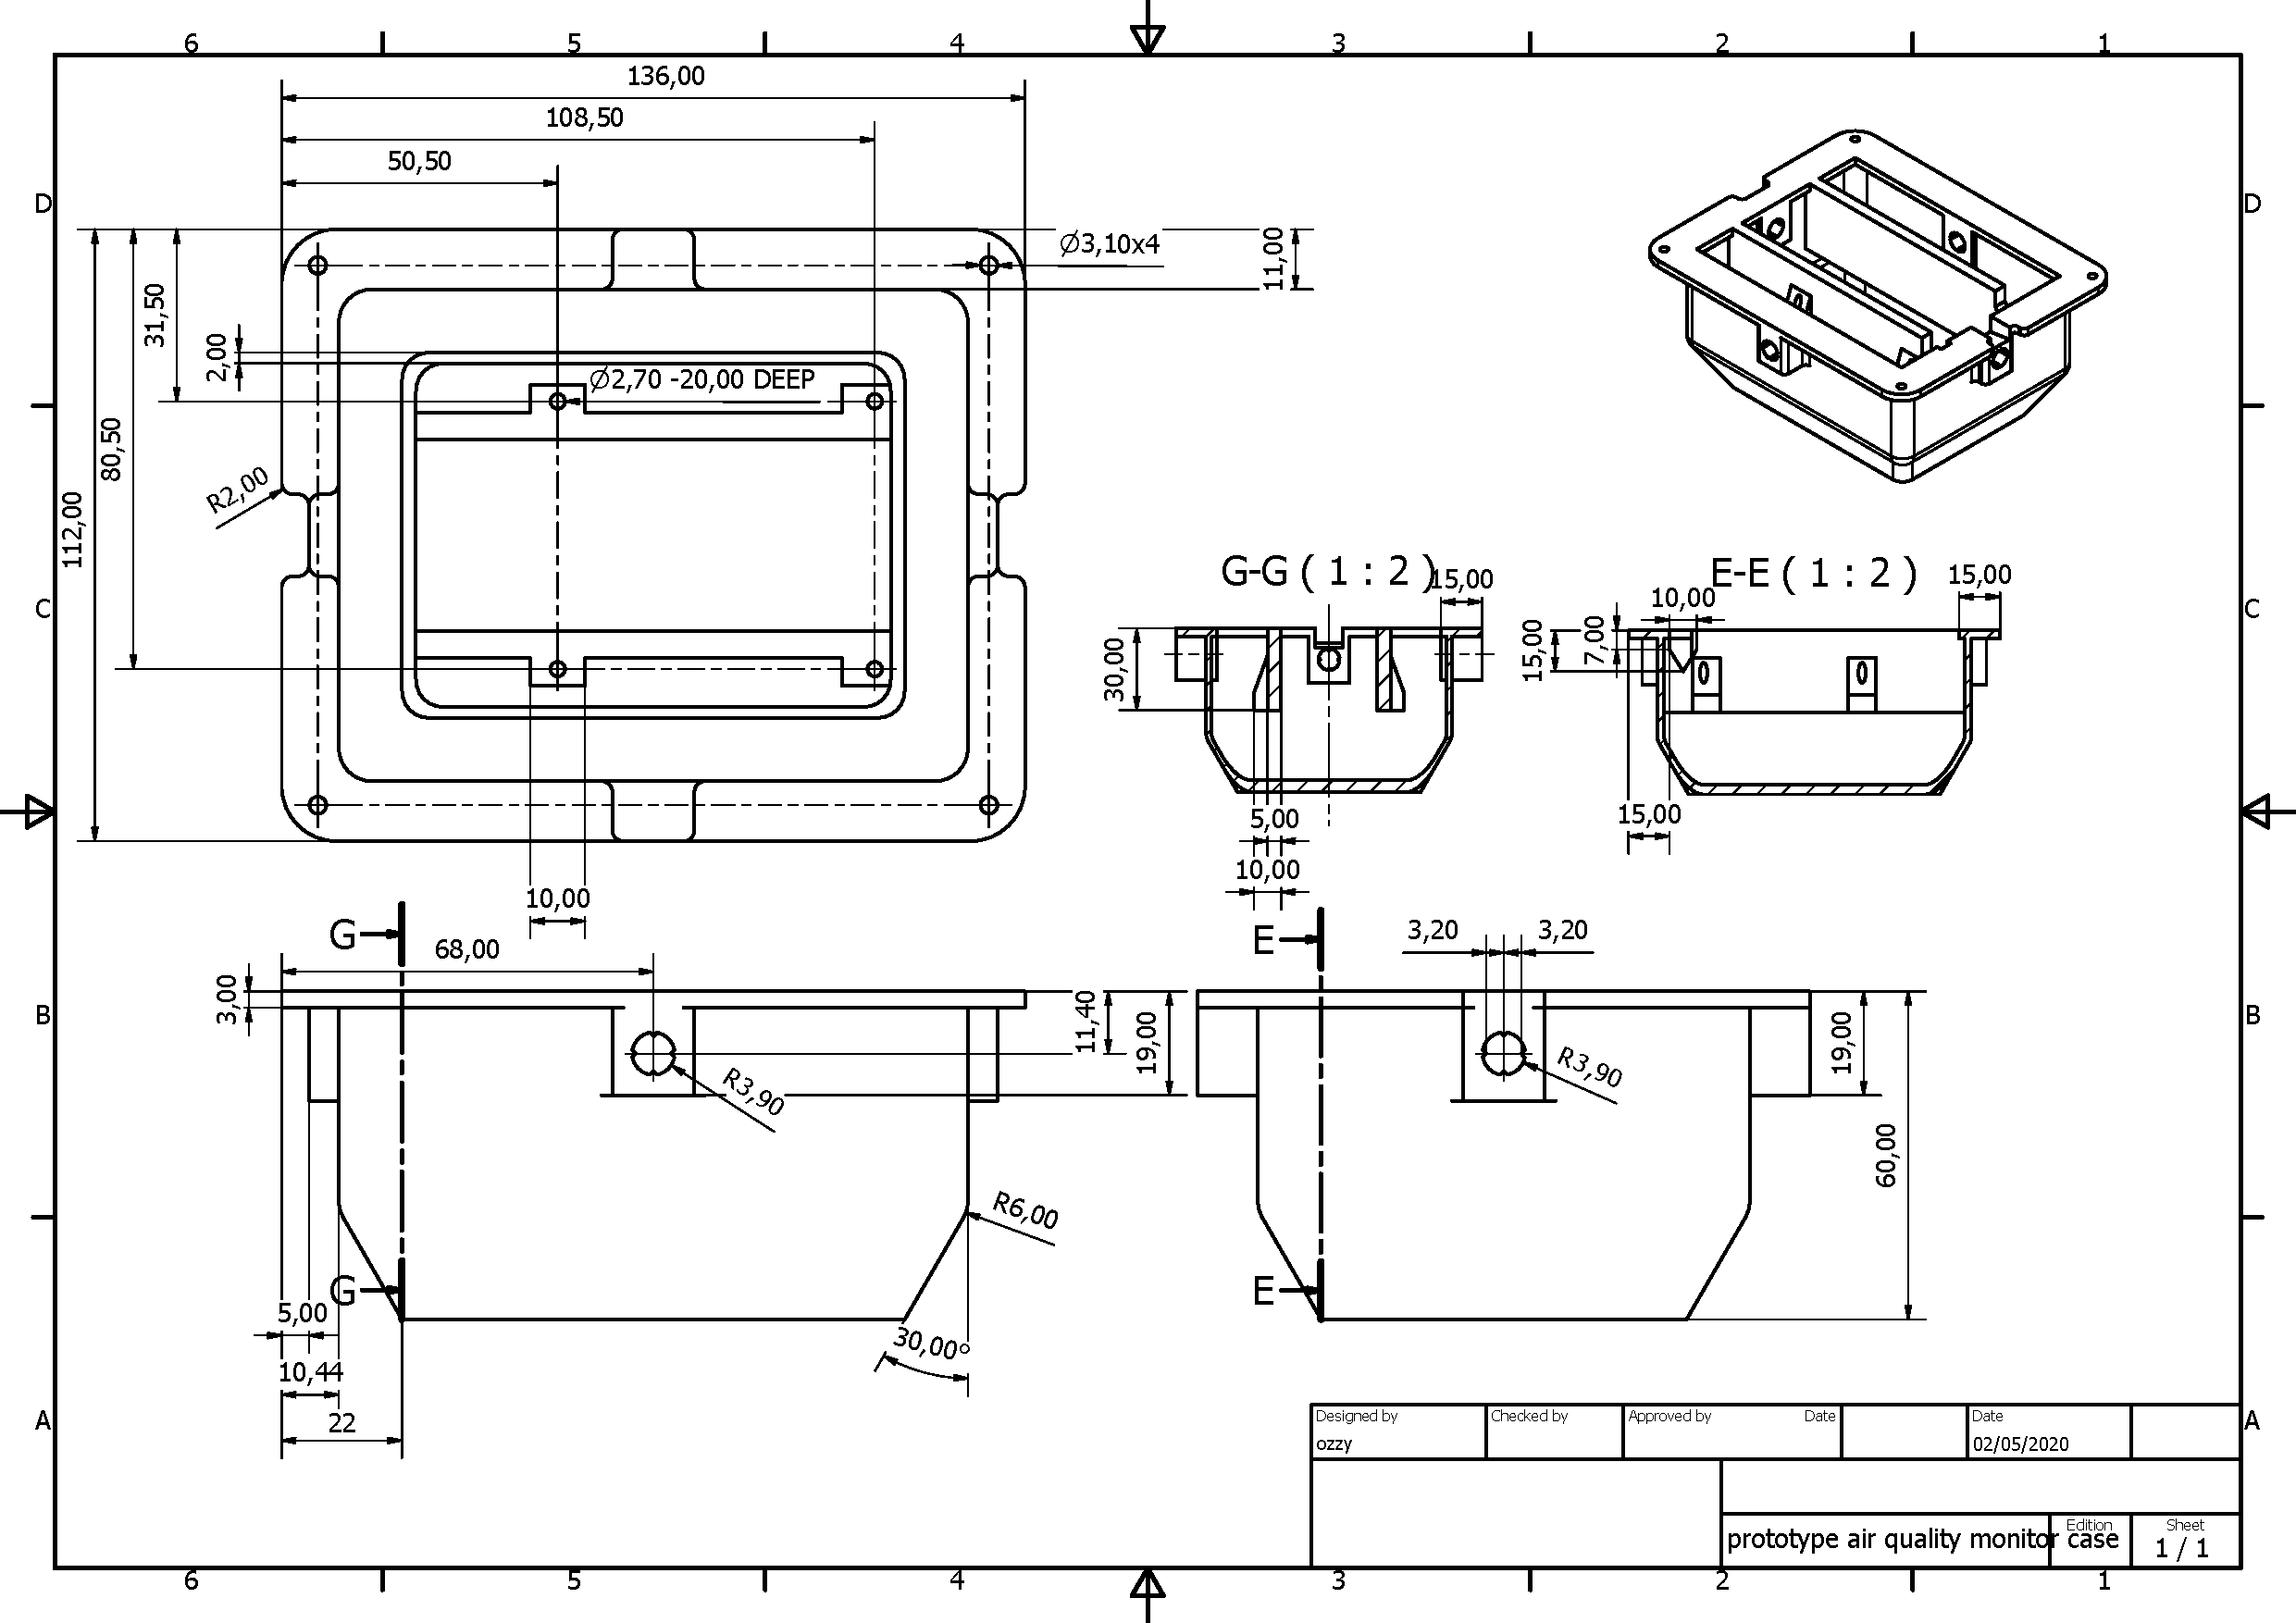
\includepdf[pages={-},fitpaper,rotateoversize]{Engineering_hardware/prototype_air_quality_monitor_case.pdf}

\textbf{Discussion}



\textbf{Final Design}

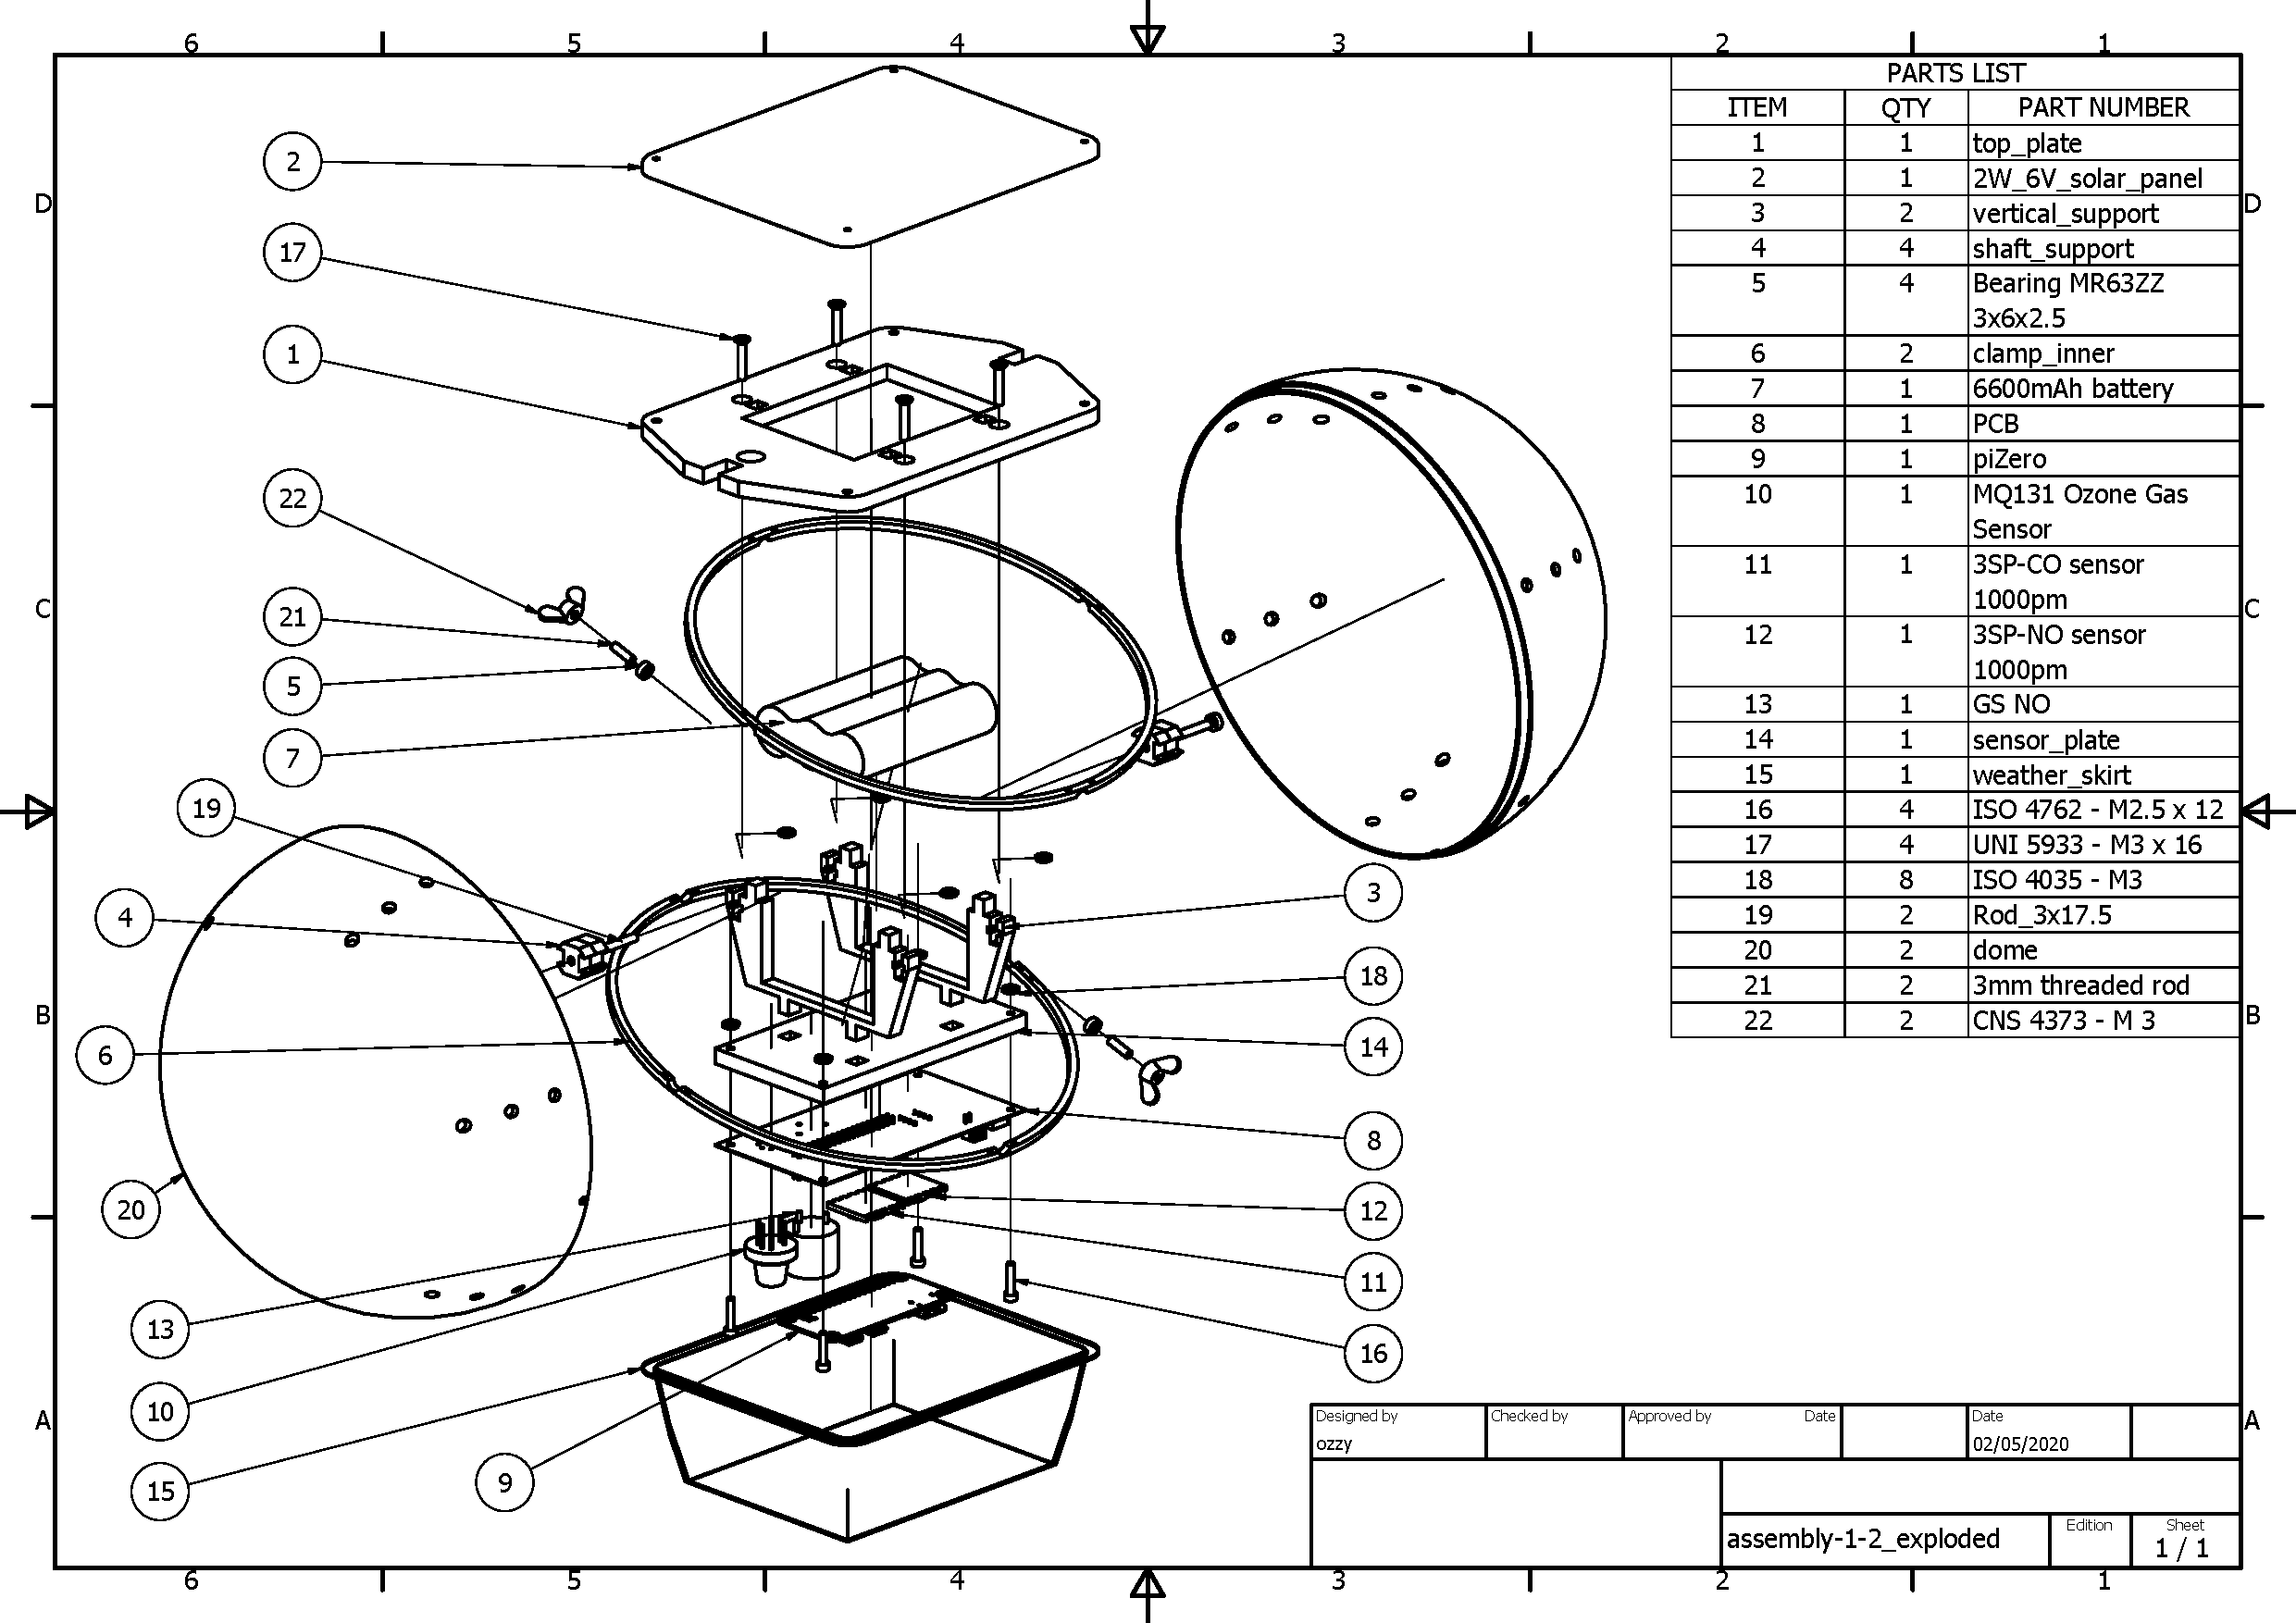
\includepdf[pages={-},fitpaper,rotateoversize]{Engineering_hardware/assembly-1-2_exploded.pdf}

\textbf{Design for Manufacture}

\textbf{Design for assembly}

Cost



cad designs

parts and cost break down?

images

review


Final Design
Short comings of prototype FEA
final design


Life Cycle Assesment